%---=---==---===---====---=====---======---=====---====---===---==---=---%
%-                  DETAILED DESIGN AND IMPLEMENTATION                  -%
%---=---==---===---====---=====---======---=====---====---===---==---=---%

\chapter{Implementation}\label{chap:implementation}

The implementation chapter involves taking the design choices made previously, and implementing them into the system. Sections covered are networking, detection, analysis, visualisation and interfacing, with each detailing how the implementation was completed. Code snippets and images are presented throughout to better explain some of the more crucial steps, however refer to the \nameandsecref{chap:code} for viewing the full code base.

\section{Networking}
The most important functions to implement for network communication are for sending and receiving data. \citet{boost} is a set of C++ libraries that support a number of tasks such as multithreading and image processing, it is also capable of cross-platform networking, and thus could be used solve the communication problem in this project. However, dependencies on libraries can bring up problems, such as complicating cross-platform building, and larger package sizes, so in an effort to keep the networking implementation small, it was decided to write the networking functions without the use of a library.

\cref{lst:recv} shows several lines of the receive function that was implemented, it takes a generic buffer, an integer length, and a number of retries as parameters. Using generics in this function makes the code more robust because it means the system has the ability to send any buffer type, for example, strings, unsigned chars and integers. Also, the function makes use of exponential backoff (\cref{lst:expbackoff}), which means that if the system attempts to send a buffer that does not get received on the other end, it will wait an ever growing amount of time before trying again. Exponential backoff is beneficial to the system because it prevents unnecessary resources from being used up when the connection between nodes is not fully realised. A backoff limit of 10000ms was chosen as it is long enough to not cause resource issues, but not too long as to cause inconvenience to the user.

\lstinputlisting[style=cpp, linerange={30-37}, label={lst:recv}, caption={Receiving network bytes in \nameandsecref{code:network}}]{code/network.hpp}

\lstinputlisting[style=cpp, linerange={51-53}, label={lst:expbackoff}, caption={Exponential backoff in \nameandsecref{code:network}}]{code/network.hpp}

In contrast, the send function (\cref{lst:send}) sends all bytes from a generic buffer. It does this by attempting to send the whole buffer at once, if the whole buffer is successfully sent in one transaction then the function returns, otherwise, if the amount of bytes sent is less than the buffer size, then the function will attempt to send whatever data is remaining, this is useful for sending large buffers of data which exceed the network protocol maximum segment size, such as images. On the other hand, if an attempt fails because the socket does not contain an open connection, the function will throw a SocketException, which will print an error such as "Failed to send all bytes of message. 4/12 of char array.". This error type was useful for debugging when writing the network functionality, because it gives the programmer a detailed description of what was being sent when the error occurred, and will continue to be useful when network problems occur in the future.

\lstinputlisting[style=cpp, linerange={59-66}, label={lst:send}, caption={Sending network bytes in \nameandsecref{code:network}}]{code/network.hpp}

Next, \textit{send} and \textit{receive} can be built on top of to create more appropriate functions, like sending and receiving images. Images in OpenCV are stored in matrices, which have a number of rows, columns and channels, for instance, an HD coloured image may be stored as a 1080x1920x3 matrix of unsigned chars. Sending a matrix first requires encoding to the Portable Network Graphics (PNG) format, which supports lossless data compression, this is good because compressed files take less time to send over a network than their sources, and also no data is lost, unlike competing compression methods such as JPEG. Then, the PNG buffer size is sent to the receiving node, so that it knows how large the matrix will be, and then finally the buffer itself is sent. On the receiving node, a simple decode of the data is required to convert back to the matrix type.

Unfortunately, compiling OpenCV with encoding functionality was not possible because of an undefined reference in the SDK, so a compromise was made which involved sending the raw matrix as continuous data, and reconstructing that matrix on the other side. This method is slower than when using compression, and therefore should only be used when the OpenCV \textit{imencode} and \textit{imdecode} functions are unavailable, like with the Android SDK.

The next step after creating the functionality for sending matrices is to handle when and how to begin communication between client and server. For instance, if the client needs to send data, then it should know that the server is ready to receive the required type of data, for this, aptly named functions \textit{sendTypeOfData} and \textit{getTypeOfData} were created. As the functions are generic, they allow for any continuous data type to be transfered, but for sake of example the list below shows the implemented process for sending an integer to the server:

\begin{enumerate}
	\item Nodes establish a connection with each other
	\item Server waits on a data type to be received
	\item Client sends the \textit{int} type to the server
	\item Server receives the \textit{int} type
	\item Server checks whether the current state of the system allows for an \textit{int} to be received
	\begin{enumerate}
		\item If an \textit{int} is acceptable, then server sends a \textit{GOOD\_REQUEST} status to the client
		\item Else, server sends a \textit{BAD\_REQUEST} status, followed by a list of valid request types, then returns to step 2
	\end{enumerate}
	\item Client sends the value of the \textit{int} to the server
	\item Server receives the \textit{int} value
	\item Server performs necessary computation with the received value
\end{enumerate}

Implementing the inter-node communication in the above way has several benefits over just sending data and hoping that it is well received on the other side. One of these reasons is that the server can validate requests, which is useful when it is expecting certain types of data, for example before the server perform localisation and mapping on camera frames, it first needs to know the camera calibration coefficients (more on this later in \cref{calib}). Therefore, if the client tries to send image data before sending its camera calibration, the server can choose to not accept that data, and notify the client that its request was unfounded. On top of this, the implementation is extendable (\cref{req:extendable}) by simply adding to the list of valid data types and implementing a function to perform on receipt of that data type.

Finally, sending images is a time-consuming task, as discussed in \cref{subsec:changingrequirements}, and must be performed asynchronously to satisfy \cref{req:comms}. In the implementation, this is done using \possessivecite{readerwriterqueue} ReaderWriterQueue library, which includes just two C++ header files that provide a single-producer, single-consumer lock-free queue. This library was used because of its compactness, and also since implementing multi-threaded operations is an incredibly subtle task, for instance, bugs can remain unseen in several runs of an application, only to appear seemingly out of nowhere later on. Using ReaderWriterQueue ensures that the operations are thread-safe because they have been tested and validated by the open source community. Now when the main thread of the client wants to send an image, it pushes that image to a queue and then immediately continues with its other tasks. At the same time, a worker thread checks the queue, and sends any new frames over to the client, thus providing the necessary asynchronous operation.

\section{\detection}
\subsection{Calibration}\label{calib}

With the client/server implementation completed, the next stage to implement is marker detection and pose estimation (\cref{req:pose}), but before marker poses can be estimated, camera-specific distortion must first be addressed (\cref{req:camera}). The implementation for which is as follows:

\begin{enumerate}
	\item Generate and print an ArUco or ChArUco board
	\item User is directed to point the camera towards the board
	\item System detects markers in each camera frame
	\begin{enumerate}
		\item If more than half of the board markers are detected, save the marker id and coordinates
		\item Otherwise, disregard the frame
	\end{enumerate}
	\item When markers for at least 10 images have had their marker coordinates saved, calibrate the camera
	\item Finally, send calibration details to the server
\end{enumerate}

The above implementation builds in two variables that are different from the standard calibration process. Firstly, the number of markers on a board to detect before saving marker coordinates is set to 1 in the \citet{aruco} sample code; however, this can lead to a high average error rate, so this system waits for at least half of the board to be detectable before saving the marker coordinates. The number of images saved before calibration is increased from 5 to 10 for the same reason; this is backed up by the \citet{ucoslam} GUI which recommends adding ten images before calibration.

The server needs to know the camera calibration coefficients because it will be performing the mapping and localisation of markers, whereas the client does not need to do this, though the client will keep hold of the calibration details for the visualisation stage later on in the pipeline.

\subsection{Dictionaries}

Next, the user is directed to choose a marker dictionary with which to detect block markers. \citet{arucopaper} proposed the ARUCO\_MIP\_36h12 dictionary because of its high inter-marker distance and therefore it is less prone to false positive detection; thus it should be used in this project. However, the OpenCV SDK that contains ArUco only supports a few dictionaries, of which the dictionary mentioned above is not among, it is instead part of the standalone ArUco library. Further, the independent and annexed versions of ArUco store dictionaries in different ways, so it requires more than a straightforward copy of data to transfer the intended marker information.

\lstinputlisting[style=cpp, linerange={27-38}, label={lst:dictionaryconversion}, caption={Dictionary conversion in \nameandsecref{code:dictionary}}]{code/dictionary.cpp}

\cref{lst:dictionaryconversion} shows a snippet of code which converts a standalone dictionary to an annexed dictionary, it does this by generating images for each marker in the source dictionary with a bit size of 1, converting the white values from 255 to 1 (\cref{fig:markerconversion}), and finally converting those bits to a byte list. Afterwards, the byte list is sent to the client where it is used to initialise an OpenCV ArUco dictionary. This method allows the client to access custom dictionaries which otherwise would not be available to it, which is worthwhile because these dictionaries have considerable benefits over those that are built-in, namely greater inter-marker distance.

\begin{figure}[ht]
\centering
\begin{minipage}{.3\textwidth}
    
\includegraphics[width=.8\textwidth]{images/implementation/aruco_mip_36h12_00000}
\end{minipage}
\tikz{\draw[->](0,0)--(2,0);}
\hspace{2pt}
\begin{minipage}{.3\textwidth}
\begin{tabular}{lllllll}
& 1 & 1 & 0 & 1 & 0 & 0 \\
& 1 & 0 & 1 & 0 & 1 & 1 \\
& 0 & 1 & 1 & 0 & 0 & 0 \\
& 1 & 1 & 1 & 0 & 1 & 0 \\
& 0 & 0 & 0 & 0 & 1 & 0 \\
& 0 & 1 & 1 & 1 & 0 & 1
\end{tabular}
\end{minipage}
\caption{A marker (left) and a generated matrix of bits (right)}
\label{fig:markerconversion}
\end{figure}
    
\subsection{Markers}

Having sent the calibration details to the server, and having chosen a dictionary, the set up is complete, and marker detection can begin. The user is directed to move their camera around the tower, as they do so the system detects markers in each frame and draws a box around them (\cref{fig:markersandmap}) depending on the map component they belong to, where a map component is a set of detected markers that have known relative positions with each other.

For instance, when the first marker is detected, it is added to a new, empty map component. When further markers are detected, the system checks to see whether any of the markers in the frame have already been added to a component, if so then they are deemed connected, and the system adds all currently detected markers to that map component (\cref{lst:findingcomponents}). If the detected marker is not linked to any other markers, then it starts its own component. For visualisation, markers in different map components are outlined in different colours, this means that the user can see which components remain unconnected, and can then position their camera in such a way to connect the components. Eventually, all the markers in the tower will be detected and connected together as one component, at this point the client ensures that all images have been sent to the server, displays a loading buffer to the user, and waits for the server to send back results from the analysis.

\lstinputlisting[style=cpp, linerange={128-136}, label={lst:findingcomponents}, caption={Finding the lowest detected component in \nameandsecref{code:native}}]{code/native-lib.cpp}


\begin{figure}[ht]
\begin{minipage}{.45\textwidth}
    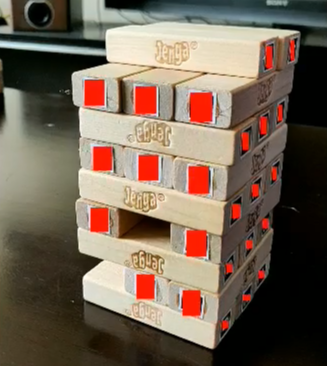
\includegraphics[width=\textwidth]{images/implementation/detection.png}
    \label{fig:detectedmarkers}
\end{minipage}\hfill
\begin{minipage}{.45\textwidth}
    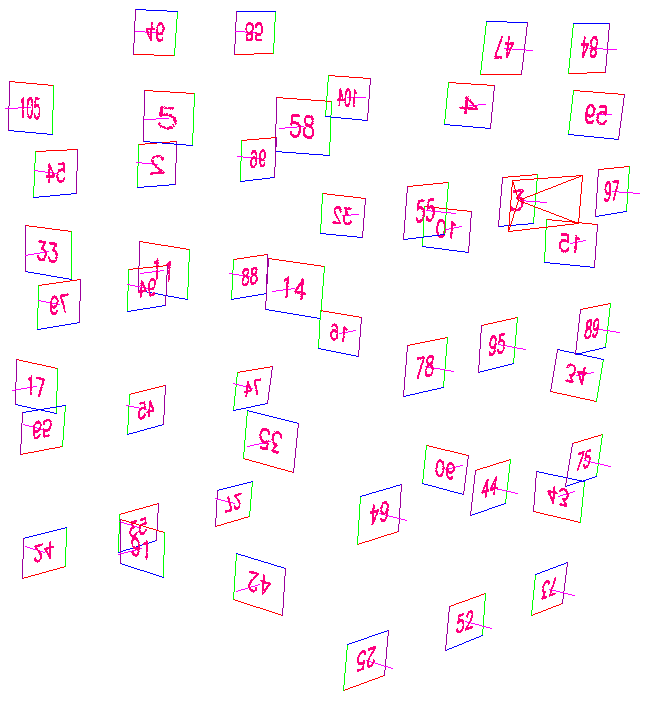
\includegraphics[width=\textwidth]{images/implementation/map}
    \label{fig:markermap}
\end{minipage}
\caption{Detected markers on image (left) and a constructed marker map (right)}
\label{fig:markersandmap}
\end{figure}

During the time that the user is scanning the tower, the client is sending images to the server whenever a new component is created, or an existing component is updated. Smartphone cameras generally capture around 30 frames per second, the majority of these frames will not contain any new information about the tower, so it makes sense to only send a subset of these images. Also, sending fewer images is more efficient and requires fewer resources from the client. Once the server has received all the images, it runs the MarkerMapper program with the camera calibration file it received earlier. The results of this can be seen in \cref{fig:markersandmap}.

The change from using UcoSLAM to using MarkerMapper was not unfounded. Advantages of using UcoSLAM were clearly defined in \cref{subsec:aruco}, however when implemented into the system UcoSLAM failed to perform to a satisfactory standard. For instance, the library resulted in segmentation faults depending on the order and content of images it processed, this means that sometimes UcoSLAM failed to produce a map of key points and markers. Clearly, this makes the library unacceptable for use at this time, however, it could quite easily be incorporated if it improves in the future. MarkerMapper is an older library that UcoSLAM was conceived from, and although it hasn't received any updates in over two years, it was able to produce a marker map with consistency, hence it is used throughout the rest of the project.
    
\section{\analysis}

\subsection{Reconstruction}

From the marker map produced earlier, a scene is built in Unity  (\cref{fig:reconstructionunity}. Marker maps are stored in the YAML 1.0 format (\cite{yaml}), which is long outdated, and while there are several YAML 1.2 libraries for deserialisation, there don't appear to be any libraries that support deserialisation for 1.0, so a short function was written to extract the relevant data and dump it into a C\# hashtable. The deserialisation task involves reading the file into a stream, splitting the stream up by certain vital characters, i.e. \{, [, :, and exporting the extracted coordinates with their corresponding marker id. These coordinates represent the three-dimensional location of the four corners of each marker.

\begin{figure}[ht]
    \centering
    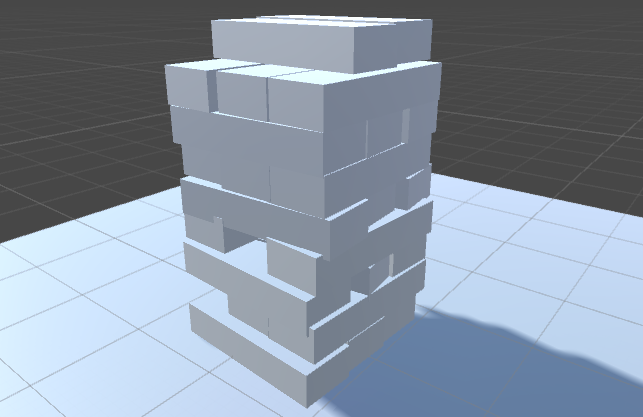
\includegraphics[width=\textwidth]{images/implementation/reconstruction}
    \caption{Reconstruction in Unity}
    \label{fig:reconstructionunity}
\end{figure}

Moving on, a Unity prefab was created to store the properties of virtual \jenga{} blocks. The dimensions of this object are variable, and can be set in the settings screen of the application, but by default, the object is set to 1.5x0.3x0.5 Unity units, this is because official \jenga{} blocks are of the same aspect ratio, and using units close to 1x1x1 makes development more manageable. Further, the object has a rigid body component attached to it, which means that the physics engine can control it, thus allowing it to be affected by collisions and gravity.

In order to instantiate the block GameObject, Unity requires a position, which indicates the centre point of the block, and a rotation, given as a Quaternion. It is clear that only knowing marker corner coordinates is not sufficient to instantiate the blocks; thus the centre point and rotation must be calculated. Finding the centre point of a block is straightforward; it involves finding the midpoint of each marker, and then finding the midpoint between those results. The algorithm used to find these midpoints can be seen in \cref{lst:midpoint}. Using midpoints of markers to calculate the centre of a block is an approximation, due to the placement of markers on real blocks being inconsistent, and also the detection and pose estimations having inaccuracies, which can cause generated objects to overlap, thus causing issues in analysis. However, it was found to be a sufficiently accurate approximation in most cases.

\lstinputlisting[style=cpp, linerange={341-344}, label={lst:midpoint}, caption={Calculating midpoints in \nameandsecref{codesec:analysis}}]{code/StandardTower.cs}

Further, a vector is calculated from the difference between the marker midpoints; this vector represents the direction that the block will be generated in. Also, for consistency, this directional vector, and the marker midpoints are all scaled to the size of the block prefab which was created earlier, thus finally allowing for the creation of the block objects. Afterwards, blocks are translated to the virtual origin so that the user can see them. Again, refer to \cref{fig:reconstructionunity} for an example of tower instantiation.

\subsection{Analysis}

Before the virtual tower can be used for analysis, its stability must first be assured; if the virtual tower were to fall over before any blocks are removed, then it would render the analysis useless. In some instances, the tower was found to sway on creation; this is because the model needs to adjust to the physics properties of the engine. To solve this motion problem, a function was devised which repeatedly waits for an in-game second, and then probes each block for information on its position and rotation, then when no blocks have moved since the last update, the tower is deemed settled;  \cref{lst:settling} shows how this algorithm was implemented in the code. Additionally, a maximum wait time of 10 seconds was decided, after which the tower is deemed to be unsettled, and the system will reject the tower state.

\lstinputlisting[style=cpp, linerange={185-193}, label={lst:settling}, caption={Waiting for settled tower in \nameandsecref{codesec:analysis}}]{code/StandardTower.cs}

Now, the removal feasibility rankings can be calculated. \cref{lst:analysis} shows that the implementation for this is quite short, yet effective. The process repeated is as follows: first, select the next block in the list and remove it, then, wait a specific amount of time, e.g. 5 seconds, next, get the sum of positional changes of every block, which is used as the score. To clean up, replace the block back into the tower and reset all blocks back to their original poses.

\lstinputlisting[style=cpp, linerange={279-293}, label={lst:analysis}, caption={Analysing removal feasibility in \nameandsecref{codesec:analysis}}]{code/StandardTower.cs}

Two key choices were made in the above implementation; how to remove the blocks, and how to calculate the score. As \citet{jengaanalysis} found, the various operations used to remove blocks from a tower affect neighbouring blocks in different ways, and that it is not possible to determine the effect that rotational moves make; for this reason, a simpler method was used, which involves simply deactivating the block in place. Furthermore, the score is calculated by finding the sum of distance travelled for each block, this works because it means moves which cause instability can be distinguished from moves that do not. It also results in a large score if the tower topples over, which is as expected.

Scores are then normalised and used to colour blocks on a scale between green and red, with green indicating ease of removal, and red the opposite. An example of this colouring can be seen in \cref{fig:analysisunity}, which shows the effectiveness of the analysis method deployed.

\vfill
\begin{figure}[ht]
    \centering
    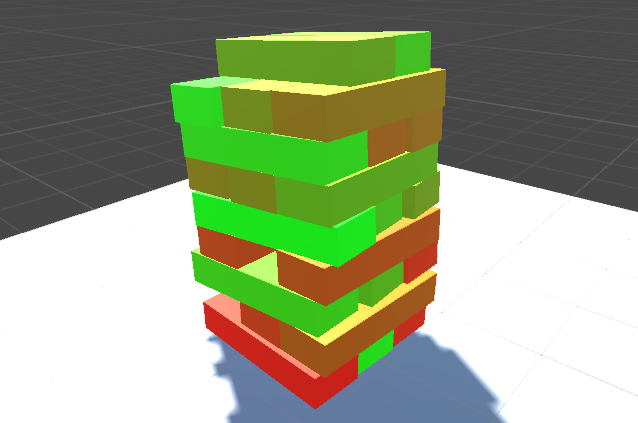
\includegraphics[width=\textwidth]{images/implementation/analysis}
    \caption{Block removal feasibility as a colour scale}
    \label{fig:analysisunity}
\end{figure}
\vfill

\section{\display}

After the scores for each block have been calculated, the next steps are to send the scores back to the client and display them. As discussed in \cref{sec:variantssummary}, the scores are displayed on a colour scale for aesthetic visualisation. This is achieved by detecting markers in each camera frame, and then drawing a box on top of each marker depending on their score. Since networking and detection functionality has already been implemented, the visualisation stage is easily attainable, requiring only normalisation of scores and drawing a filled, coloured rectangle using OpenCV. The resulting display is seen in \cref{fig:display}.

\vfill
\begin{figure}[ht]
    \centering
    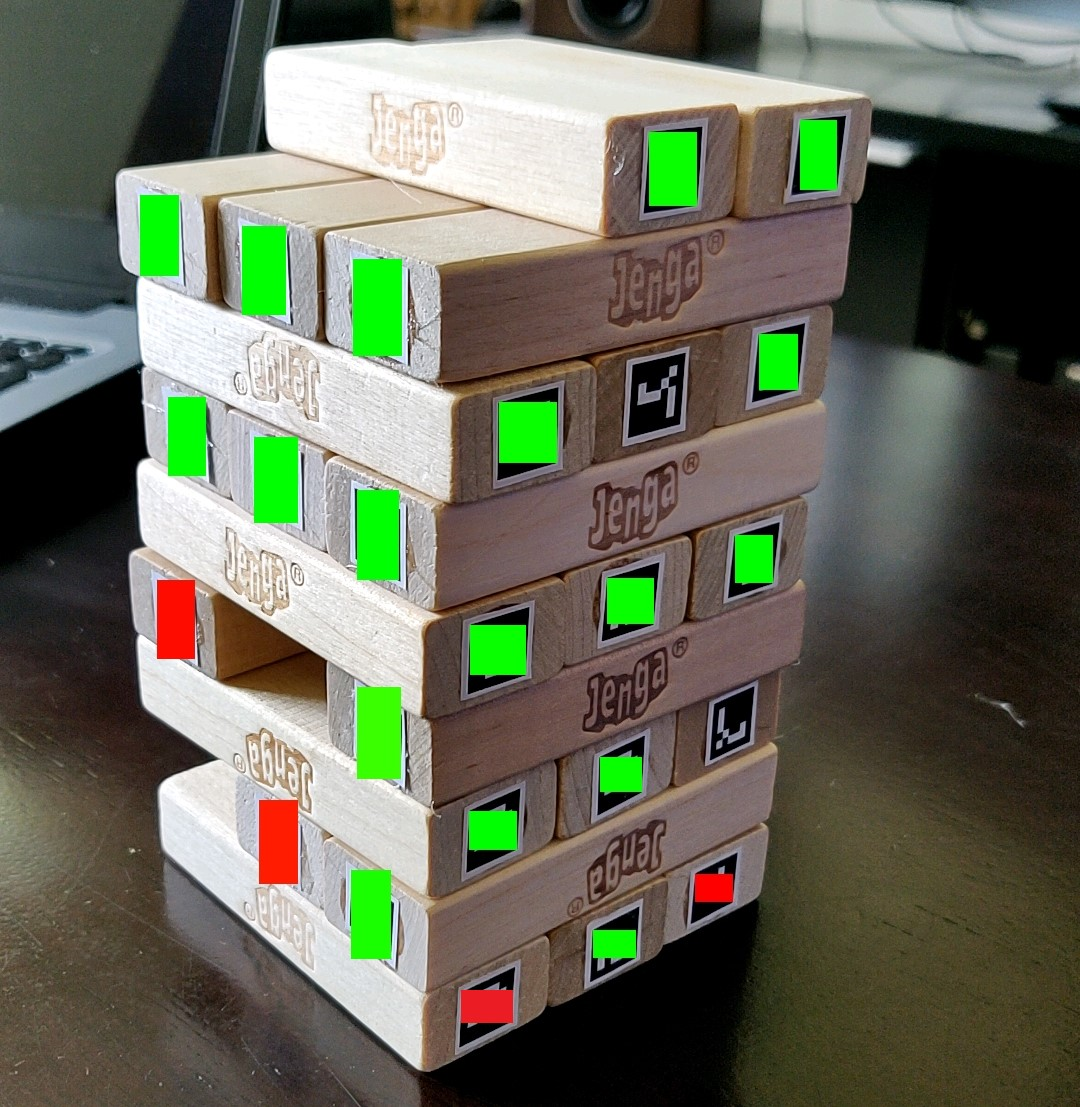
\includegraphics[width=.7\textwidth]{images/implementation/display}
    \caption{Visualisation of scores}
    \label{fig:display}
\end{figure}
\vfill

\newpage\section{Interfacing}

\begin{wrapfigure}{r}{5.5cm}
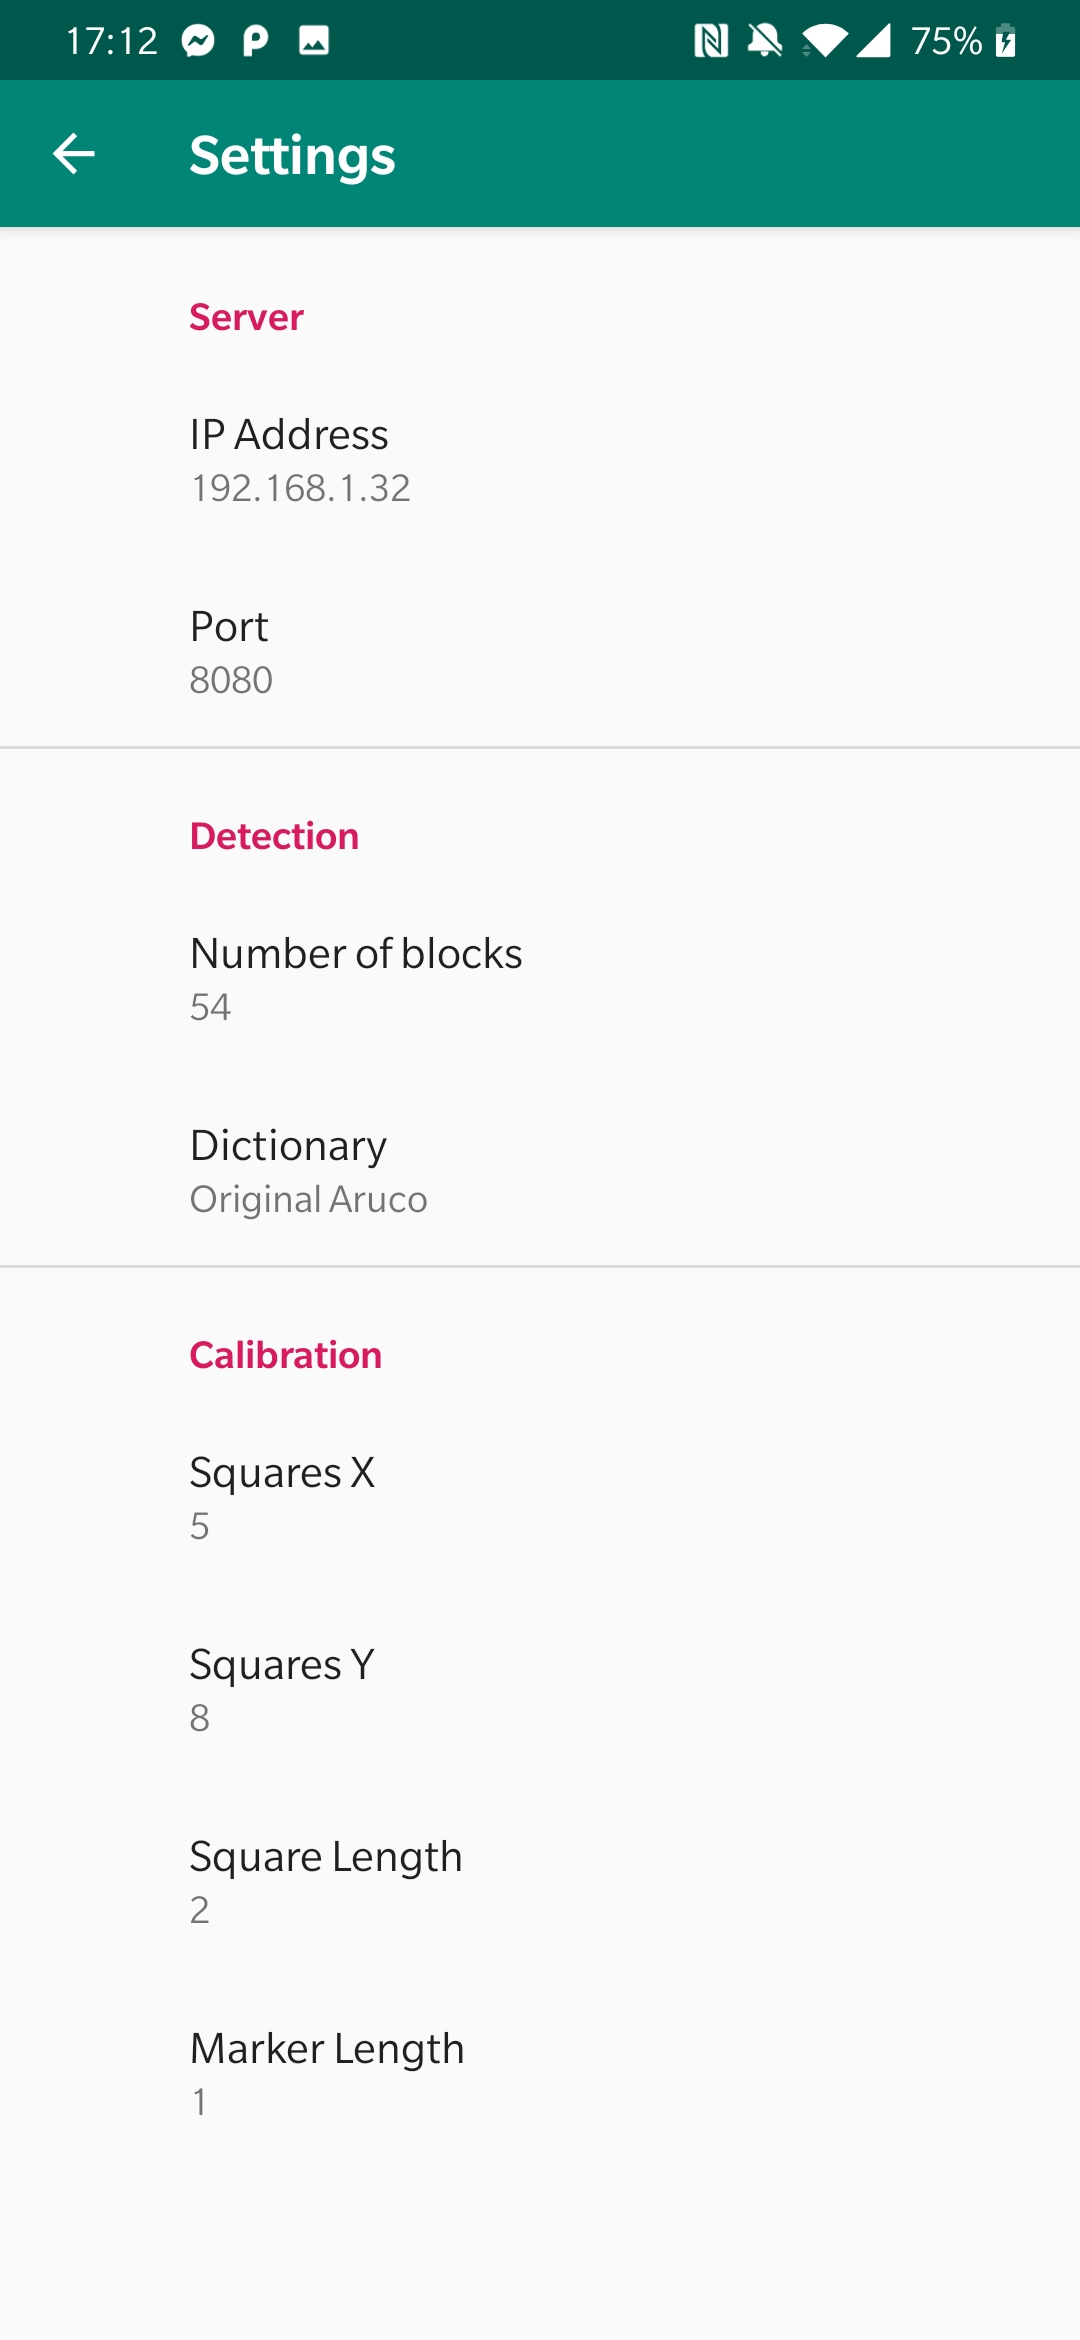
\includegraphics[width=4cm]{images/implementation/settings}
\caption{Settings screen}\label{fig:settings}
\end{wrapfigure}

When implementing the settings screen from the design section (\cref{sec:standalone}), it became clear of several drawbacks of the intended design. Firstly, the screen was missing some vital options, such as server address and port, and preferences for camera calibration. It is essential that these are included in the implementation because the server used by each user is likely to be running on a different address.

\cref{fig:settings} shows what the final implementation for the settings screen looks like. This design makes use of the Android preferences layout, which inflates a number of settings into a visually pleasing, scrolling window, which is better than previous iterations of design because of its consistency of layout and colour scheme. The previous design included a large button with which to enter the camera activity, but this was removed in favour of a back arrow, which conforms with the rest of the design for the settings.

\section{Additional GUI}

Whilst scanning the tower in to the system using fiducial markers has its benefits, it still requires the user to stick markers to both ends of each \jenga{} block, which is a monotonous task and therefore off-putting. Instead, an alternative was devised with which the user can build a virtual tower without the need for markers.

\cref{fig:towerbuilder} shows the different functionality that was implemented for such a system. When the user opens the application, they are greeted with an array of end and side blocks which appear to be in the shape of a tower. An effort was made to ensure these blocks looked realistic, in fact, the images used for the blocks were taken from a real set of \jenga{}, and then colourised and shaped to work with the application. Further, the user is able to zoom in and out, to see the full tower, or focus on a specific section for block removal. Or, the user can rotate the tower to view a different face.

The user is directed to tap on blocks in the application in the order that they were removed in the real tower; tapped blocks move from their position to the top of the tower, just as they would in the real game. By default, moved blocks go to the top left position, but can be moved to the centre, or top right, by simply clicking on them again.

While the tower is represented in a two-dimensional space, it retains a sense of realism due to the aesthetics of the blocks. This method for building the tower is beneficial because it is faster than the marker method, but its main drawback is that is doesn't account for rotation or translation of blocks; that is, blocks are assumed to be perfectly aligned in their position of the tower. Furthermore, this tower building activity was developed to be modular (\cref{req:modular}), which means that it is possible to swap out out the marker detection stage for this tower building activity, should the user choose to do so.

\begin{figure}[ht] % "[t!]" placement specifier just for this example

\hspace*{\fill}
\begin{subfigure}{0.22\textwidth}
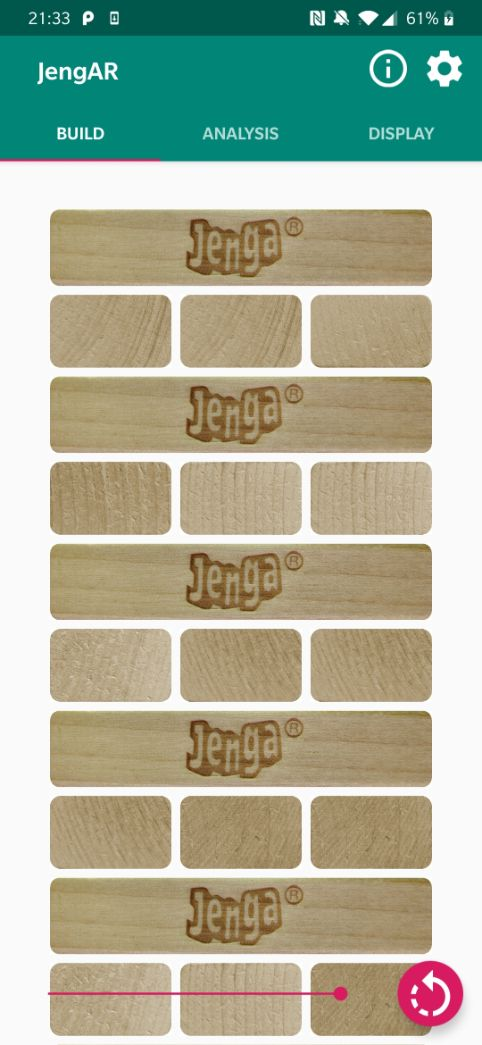
\includegraphics[width=\linewidth]{images/implementation/build-start}
\caption{Start} \label{fig:buildstart}
\end{subfigure}
\hspace*{\fill}
\begin{subfigure}{0.22\textwidth}
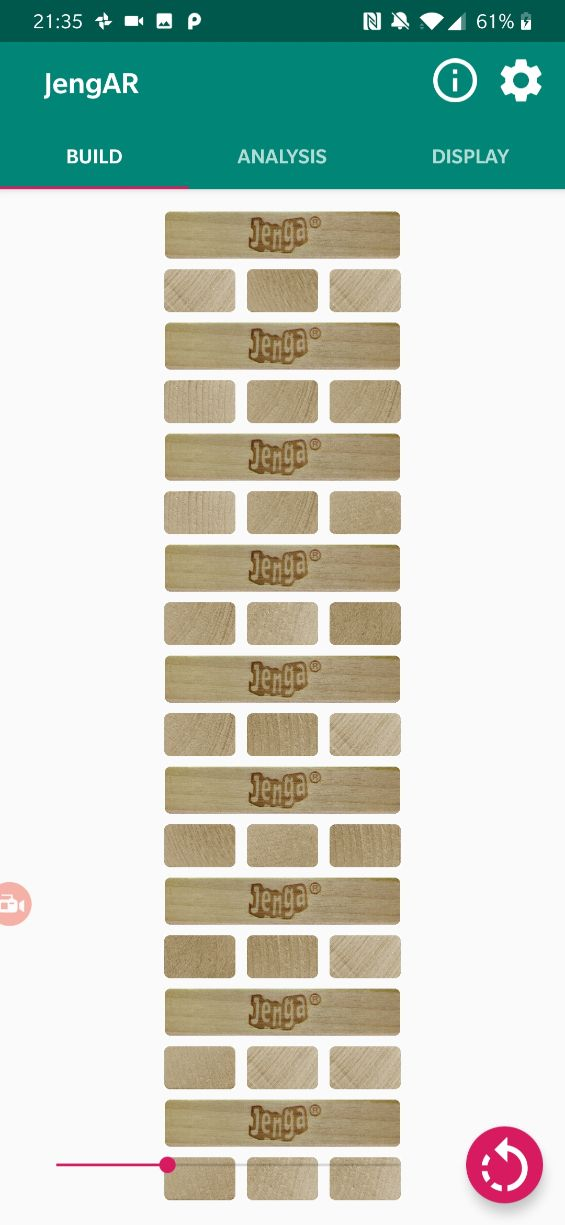
\includegraphics[width=\linewidth]{images/implementation/build-zoom}
\caption{Zoom} \label{fig:buildzoom}
\end{subfigure}
\hspace*{\fill}
\begin{subfigure}{0.23\textwidth}
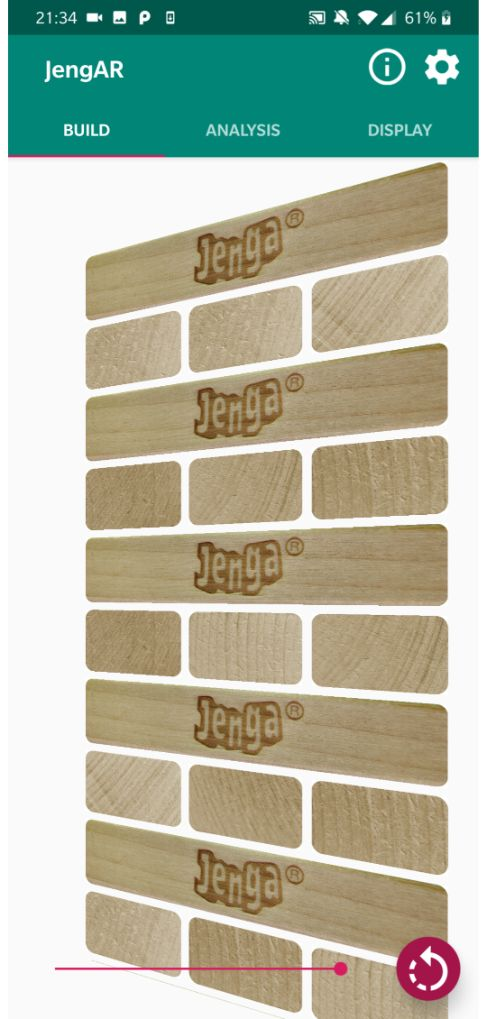
\includegraphics[width=\linewidth]{images/implementation/build-rotate}
\caption{Rotate} \label{fig:buildrotate}
\end{subfigure}
\hspace*{\fill}
\begin{subfigure}{0.22\textwidth}
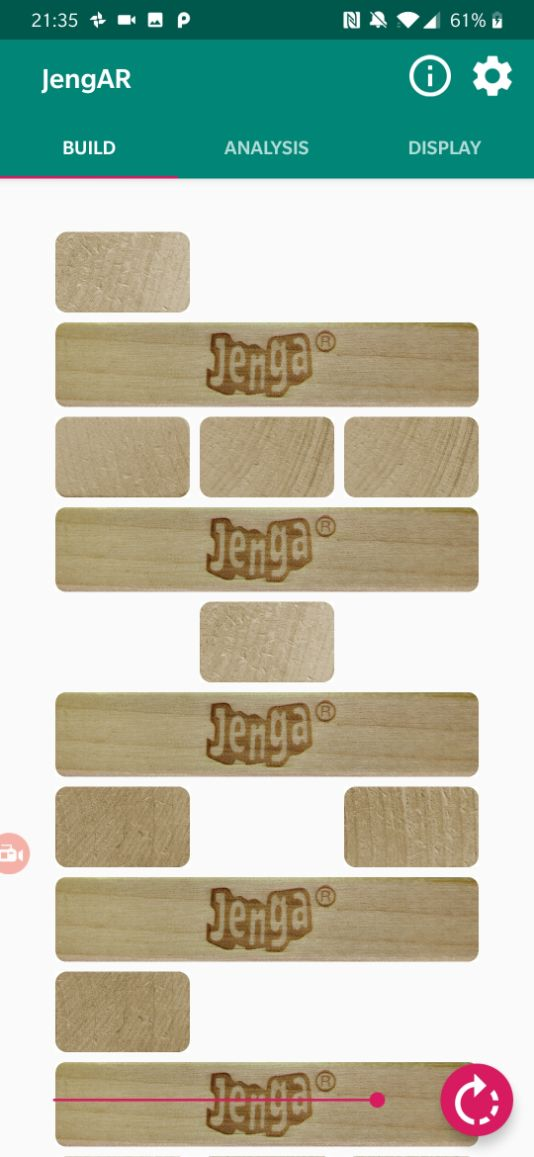
\includegraphics[width=\linewidth]{images/implementation/build-end}
\caption{End} \label{fig:buildend}
\end{subfigure}
\hspace*{\fill}
\caption{Tower builder}
\label{fig:towerbuilder}
\end{figure}

\section{Summary}

The implementation chapter has shown how the system was implemented, from the development of networking functionality, through each stage of the project, leading to a working program that displays block removal feasibilities to the user. It also introduced an alternative for tower building, if the user does not want to attach markers to their blocks. For the sake of completeness, \cref{fig:pipeline} displays the whole pipeline of the project.

\begin{figure}[p] % "[t!]" placement specifier just for this example

\hspace*{\fill}
\begin{subfigure}{0.3\textwidth}
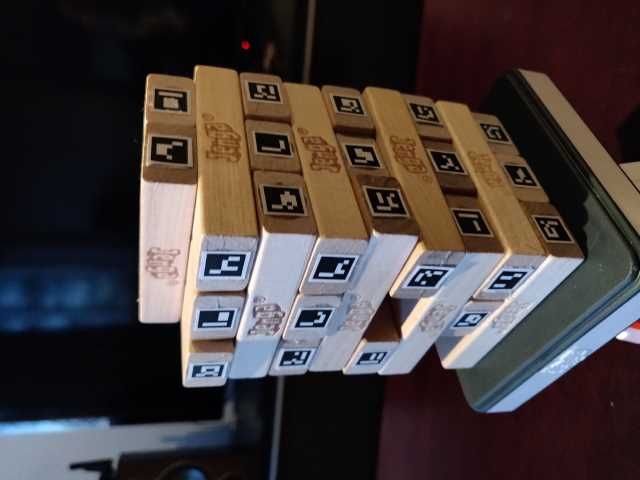
\includegraphics[angle=270,origin=c,width=\linewidth,keepaspectratio]{images/implementation/tower}
\caption{Tower state} \label{fig:a}
\end{subfigure}
\hspace*{\fill}
\begin{subfigure}{0.3\textwidth}
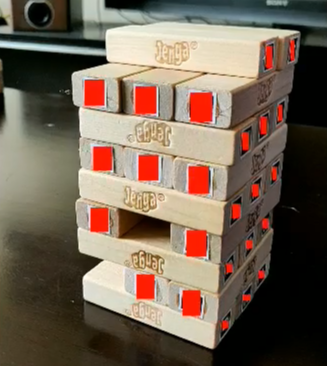
\includegraphics[width=\linewidth,keepaspectratio]{images/implementation/detection}
\caption{Detection} \label{fig:b}
\end{subfigure}
\hspace*{\fill}

\medskip

\hspace*{\fill}
\begin{subfigure}{0.3\textwidth}
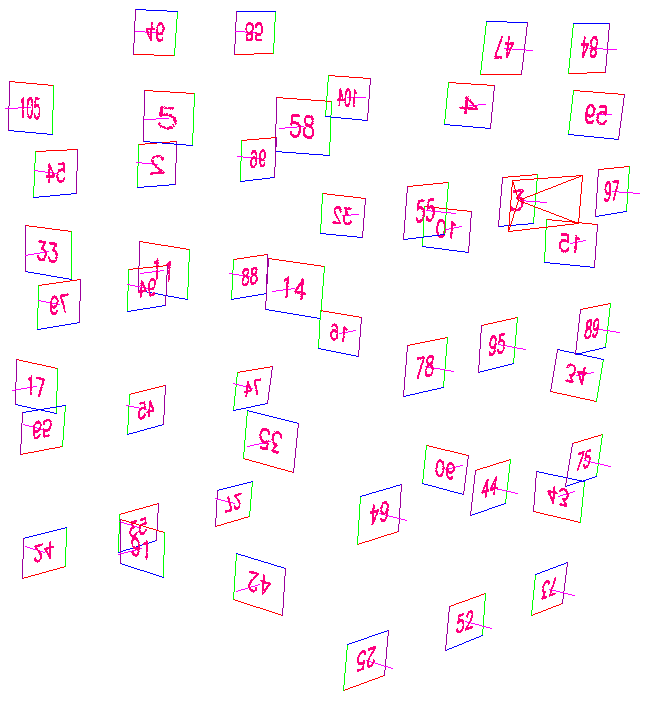
\includegraphics[width=\linewidth,keepaspectratio]{images/implementation/map}
\caption{Marker map} \label{fig:c}
\end{subfigure}
\hspace*{\fill}
\begin{subfigure}{0.3\textwidth}
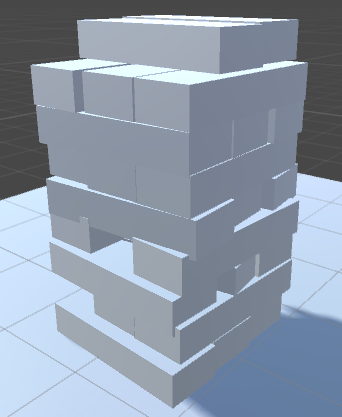
\includegraphics[width=\linewidth,keepaspectratio]{images/implementation/reconstructionportrait}
\caption{Reconstruction} \label{fig:d}
\end{subfigure}
\hspace*{\fill}

\medskip

\hspace*{\fill}
\begin{subfigure}{0.3\textwidth}
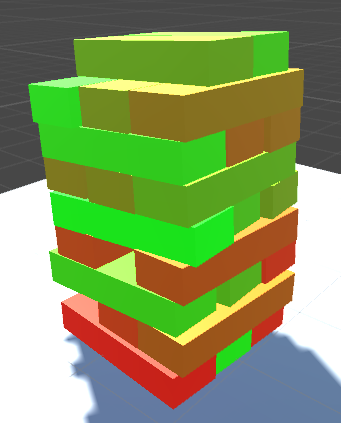
\includegraphics[width=\linewidth,keepaspectratio]{images/implementation/analysisportrait}
\caption{Analysis} \label{fig:e}
\end{subfigure}
\hspace*{\fill}
\begin{subfigure}{0.3\textwidth}
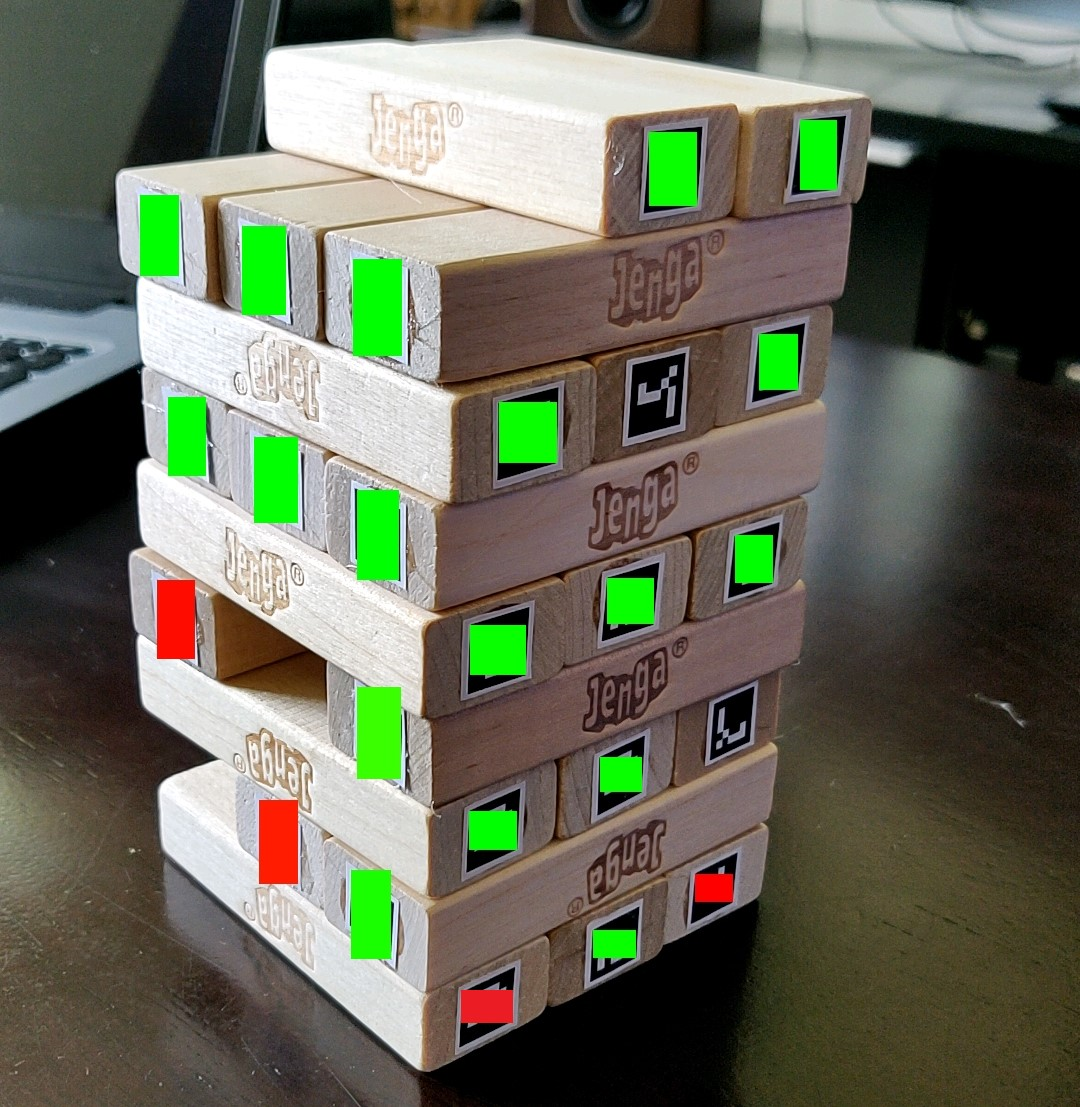
\includegraphics[width=\linewidth,height=200pt,keepaspectratio]{images/implementation/display}
\caption{Visualisation} \label{fig:f}
\end{subfigure}
\hspace*{\fill}

\caption{System pipeline} \label{fig:pipeline}
\end{figure}